\chapter{Assembly Plan and Design Verification}

\section{Design and Development Plan}

The design is scheduled to be completed on March 1st, 2022, to allow for a one-month testing and verification period. The design deliverables of the project will require a full-scale working model, which does not include a system prototype. The assembly of the project will be split into 5 parts:

\medskip
\begin{enumerate}[itemsep=3mm, parsep=-1mm, label=\roman*.]
    \item Solar Thermal Collector.
    \item Piping.
    \item System Frame.
    \item Refrigerant.
    \item Data Acquisition System.
\end{enumerate}

\medskip
The Solar Thermal Collector will consist of a glass pane, absorber plate, serpentine piping manifold, and insulation, all enclosed in a plywood frame. The assembly of the thermal collector - i.e., the brazing of the serpentine manifold onto the bottom of the absorber plate - will take place concurrently with the piping fitments into the main components (i.e., compressor, condenser, expansion valve, and collector). The piping will also be welded or brazed between the components. After the frame is constructed, and the heat pump is assembled, the system can be charged with the refrigerant. As the handling and charging of refrigerants requires qualifications, three methods will be explored: 

\medskip
\begin{enumerate}[itemsep=3mm, parsep=-1mm, label=\roman*.]
    \item Support from the maintenance team at the University of Calgary will be requested to charge the system. 
    \item Support from the refrigerant training program at the Southern Alberta Institute of Technology will be requested to charge the system. 
    \item If the aforementioned strategies fail, HVAC (heating, ventilation, and air conditioning) companies will be contacted through referrals to charge the refrigerant.
\end{enumerate}

\medskip
Finally, temperature and pressure sensors for the data acquisition system will be integrated into the piping of the system to allow for the gathering of data validation metrics such as the system coefficient of performance. The temperature probes will be inserted into brazed pockets in the piping, and the pressure sensors will be screwed into the piping through specialized T-connectors.

\section{Design Verification}

To verify the design and determine the system performance, a data acquisition system was developed.

\medskip
The performance of the design can be quantified by two parameters: the $COP$ of the system and the outlet temperature of the water.

\medskip
The $COP$ of the system can be defined as:
\begin{align}
    COP = \ddfrac{Q_{out}}{W_{cycle}} = \ddfrac{\dot m (h_2 - h_3)}{\dot m (h_2 - h_1)} = \ddfrac{(h_2 - h_3)}{(h_2 - h_1)}
\end{align}

\medskip
As evidenced by Equation 4.1, the $COP$ of the system can be determined knowing the specific enthalpy of the refrigerant at certain points. Specific enthalpy at any location can be found through use of temperature and pressure measurements and the refrigeration table of R-410A [18]. As so, temperature sensors at 3 locations (1, 2, 3) and pressure sensors at 2 locations (1, 2) on Figure 4.1 below will be used to determine $COP$. The pressure sensor at 3 can be neglected under the isobaric condensation assumption. However, a temperature sensor at 3 is still necessary as it is pertinent to know and minimize the degree of subcooling at the inlet of the electronic expansion valve. Additionally, pressure transducers are approximately at least 20 times more expensive than a thermistor at any given location, so the isobaric assumption was also used for economic reasons.
In the above $COP$ equation, it was assumed that all the power input into the compressor is going into superheating the refrigerant. This in fact is not valid, as the compressor itself will hold an efficiency factor. This efficiency factor dictates how much power the compressor puts into the refrigerant, from the total power it uses.

\medskip
To evaluate this efficiency factor, the following equation will also be used to determine $COP$:
\begin{align}
    COP = \ddfrac{Q_{out}}{W_{cycle}} = \ddfrac{\dot m(h_2 - h_3)}{W_{cycle}}
\end{align}

\medskip
To determine COP using Equation 4.2, the mass flow rate of the refrigerant and the power consumption of the compressor must additionally be known. The mass flow rate of the refrigerant only needs to be measured at one location, as per the laws of continuity. A turbine flow meter will be used at location 1 for this purpose. Additionally, a power meter will be connected to the compressor to determine power usage.

\medskip
The second parameter that will be used for design verification will be the water outlet temperature. As per the design goals, the aim is to have this temperature be 55\textdegree C. A thermistor will be paced at this location to measure this parameter.

\medskip
Figure 4.1 below provides a visual guide of sensor placements in the system.

\medskip
\begin{figure}[H]
    \centering
    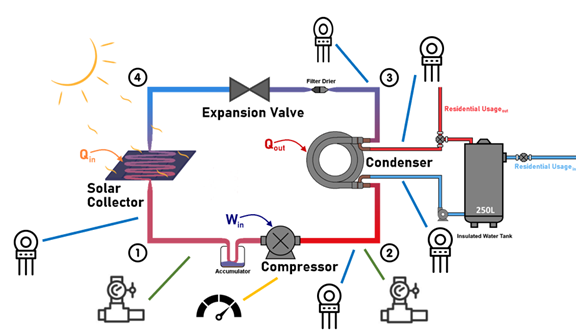
\includegraphics[width=\textwidth]{images/sensor_locations.png}
    \caption{Sensor Locations}
\end{figure}

\subsection{Data Acquisition Configuration}

To get the data outputs from the sensors, several data acquisition configurations were explored. Ultimately, an Arduino Uno was decided upon as the data acquisition device as it was the most economical option. Arduino Uno’s have only six analogs to digital converter (ADC) pins, whereas at least eight ADC pins would have been needed if all selected sensors gave analog outputs. To bypass this issue, digital thermistor sensors that could be connected to digital pins on the Arduino were chosen instead. Arduino Uno ADC pins have a maximum bit size of 12, which can affect resolution of the measurement picked up. For all the analog sensors chosen, this resulted in the smallest magnitude that could be measured being 1-2\% of the expected value. This resolution was decided to be sufficient for the needs of the data acquisition system. Table 4.1 shows a full list of sensors used. Note that the location numbering refers to schematic in Figure 4.1.

\medskip
\begin{table}[H]
\centering
\caption{List of Sensors to be used in Data Acquisition System}
\rowcolors{2}{gray!20}{white}
\begin{tabular}{|P{26mm}|P{26mm}|P{15mm}|P{27mm}|P{23mm}|P{20mm}|}
    \hline
    \rowcolor{orangeRed}
    Sensor Type & Location(s) & Accuracy & Operating Range & Power Supply & Output Type \\
    \hline
    Thermistor \cite{thermometer}            & 1, 2, 3, Water Outlet        & $\pm \SI{0.5}{\celsius}$ & $\SI{-55}{\celsius}$ to $\SI{125}{\celsius}$ & Arduino  & Digital \\
    Pressure Transducer \cite{pressure_transducer1}   & 1                            & 0.25\%                   & $0psi$ to $150psi$ & $9V$ to $30V$ DC at $<10mA$ & Analog $0V$ to $5V$ DC \\
    Pressure Transducer \cite{pressure_transducer1}   & 3                            & 0.25\%                   & $0psi$ to $1000psi$ & $9V$ to $30V$ DC at $<10mA$ & Analog $0V$ to $5V$ DC \\
    Volumetric Flow Meter \cite{pressure_transducer2} & 2                            & 3\%                      & 1L/min to 10L/min & 3.75E-5 & Amplified Square Wave \\
    Power Meter \cite{power_meter}           & Compressor Electrical Outlet & 3\%                      & 0KWH to 9999KWH & Compressor Power Supply  & Screen Display \\
    \hline
\end{tabular}
\end{table}

\medskip
All sensors will be tested and configured individually as per their respective manufacturers’ guidelines. An external power supply will be used for all sensors that require it. For more information on the different sensors that were explored, please see the Sensor Selection excel file in the Design Binder.

\medskip
To verify the design, a $COP > 2.3$ and a water outlet temperature of 55\textdegree C needs to be constantly achieved, as per design requirements. The previously described data acquisition system will assist in quantifying design verification.
